
\documentclass{scrreprt}

\usepackage{listings}
\usepackage{graphicx}

\begin{document}

\title{UO Praktikum 1}

\author{Andreas Krohn, Benjamin Vetter}

\lstset{
  breaklines=true,
  language=SQL,
  basicstyle=\ttfamily,
  showstringspaces=false
}

\maketitle

\chapter{Teil A}

\begin{figure}[h]
  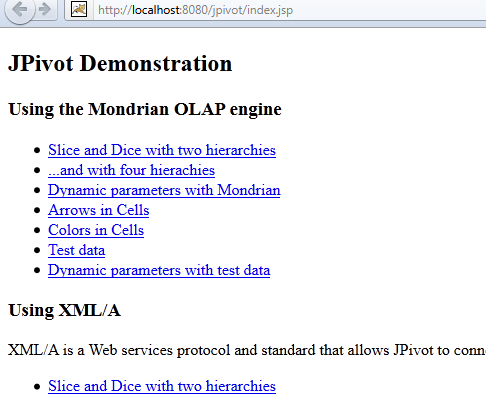
\includegraphics[width=\textwidth]{screenshots/jpivot.png}
  \caption{JPivot}
\end{figure}

\chapter{Teil B}

\begin{figure}[h]
  \centering
  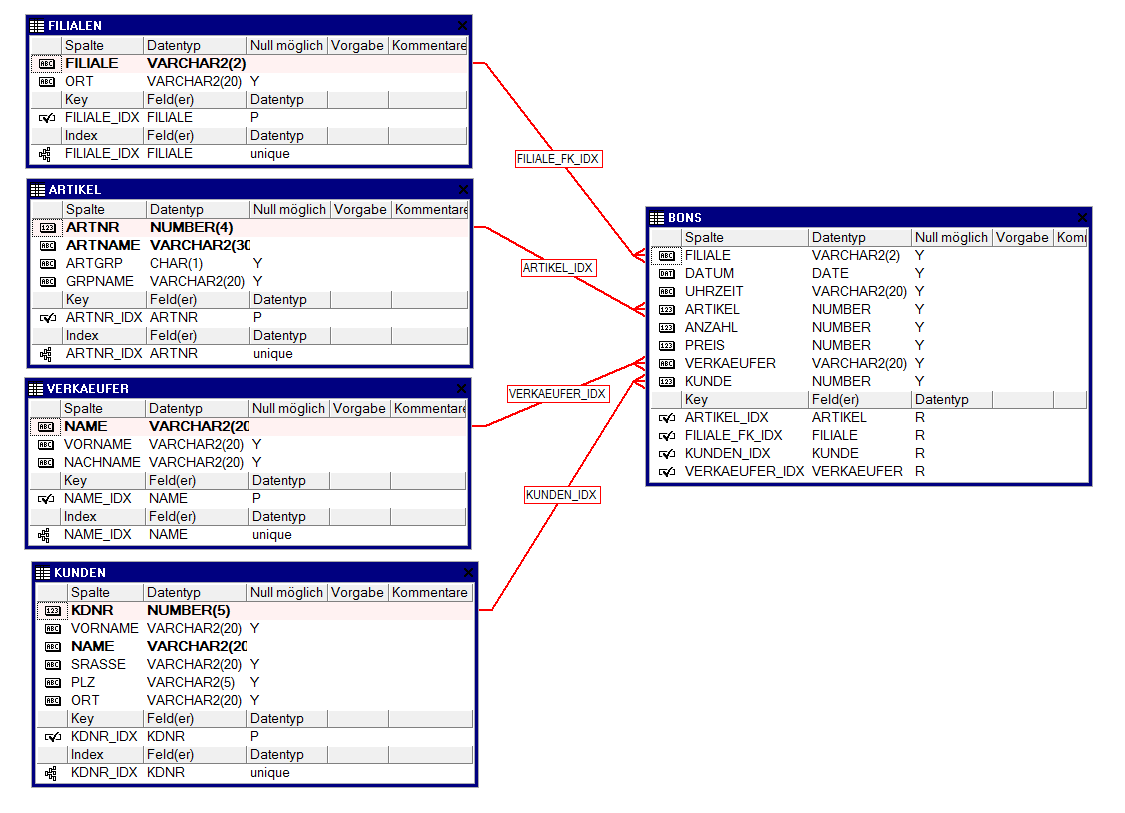
\includegraphics[width=\textwidth]{screenshots/erm.png}
  \caption{ERM}
\end{figure}

\begin{description}
  \item[Fehlerhafte Datensätze:] Die Bondatei enthält Datensätze deren Foreign Keys für Artikel, Kunden, etc. nicht vorhandene Primärschlüssel referenzieren.
  \item[Unsere Lösung:] Die entsprechenden Foreign Keys auf NULL setzen.
\end{description}

\begin{figure}
  \centering
  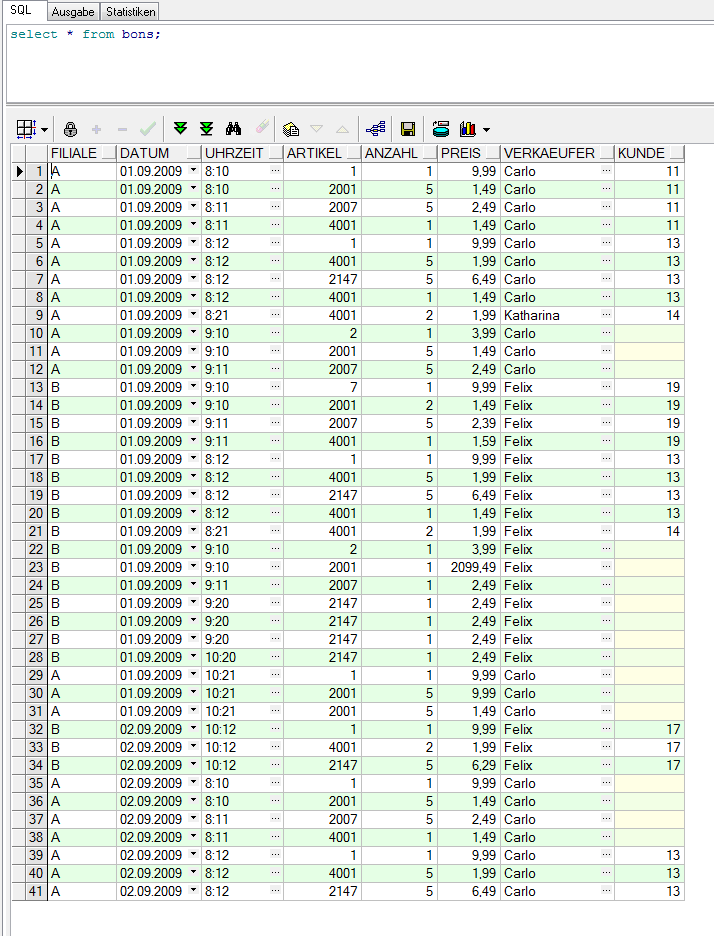
\includegraphics[width=\textwidth]{screenshots/bons.png}
  \caption{Tabelle Bons}
\end{figure}

\begin{figure}
  \centering
  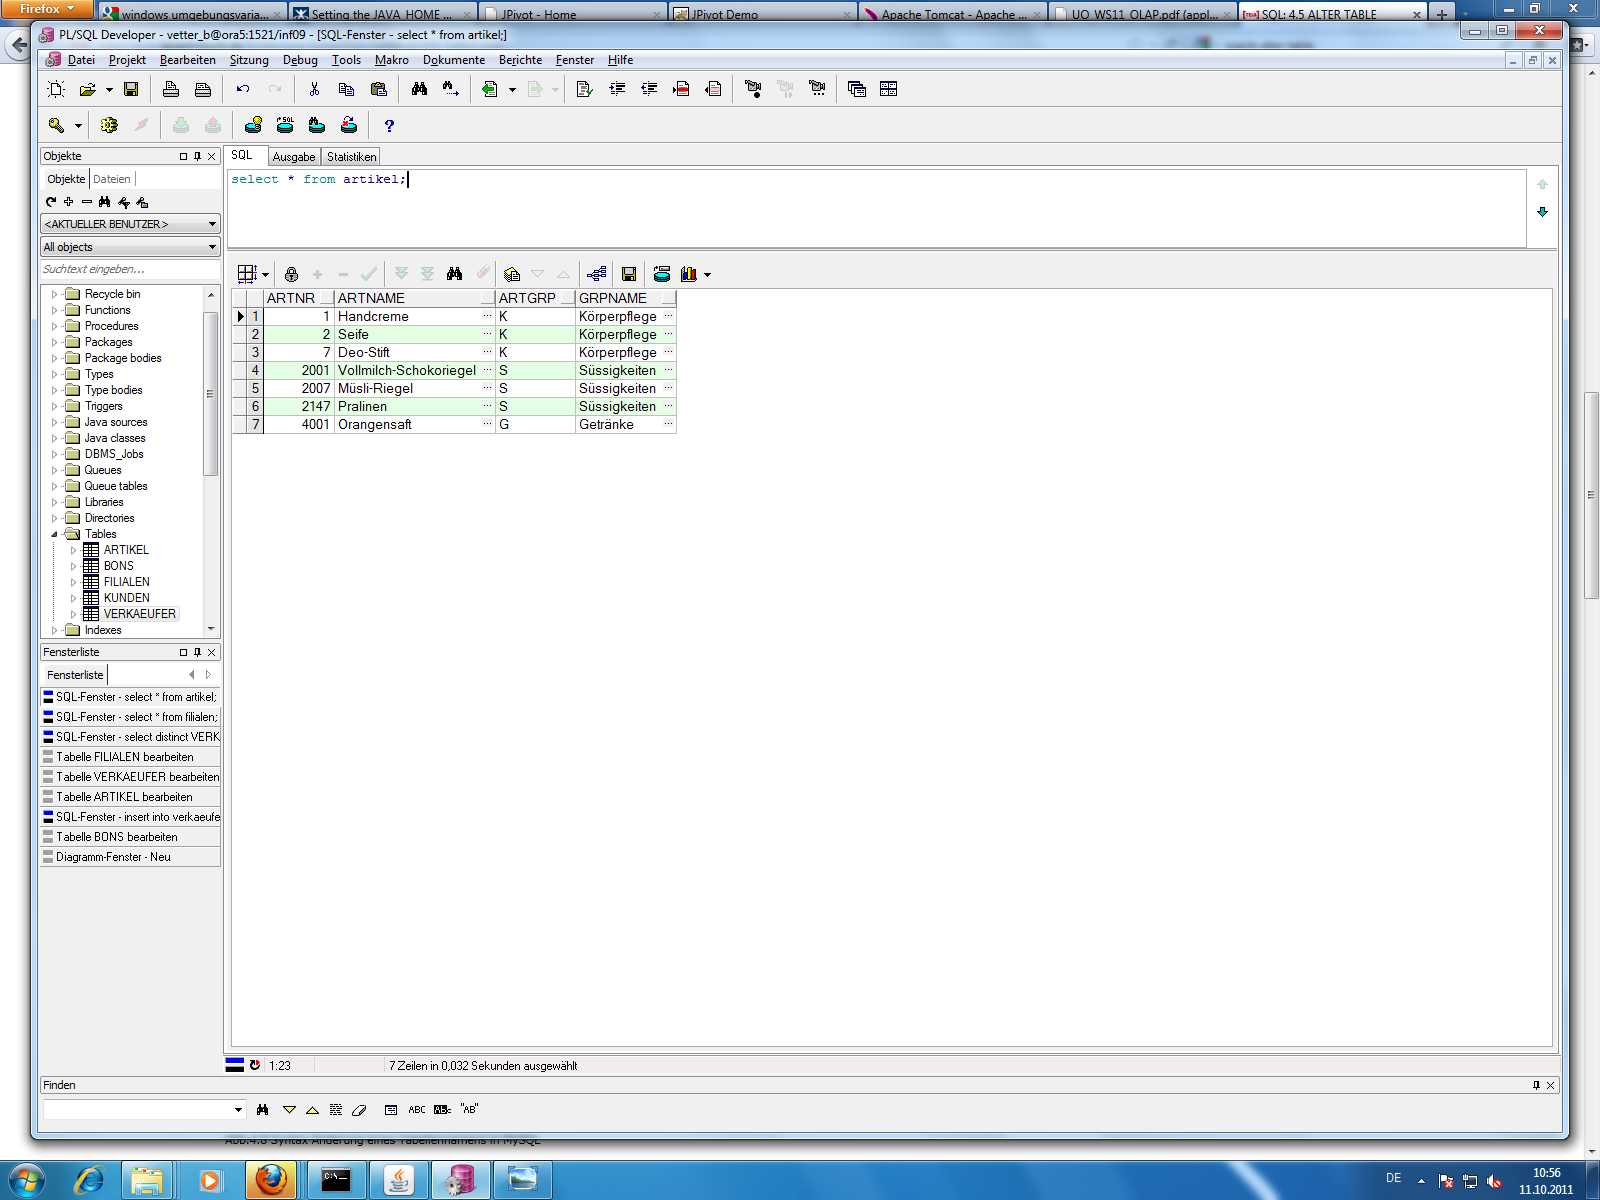
\includegraphics{screenshots/artikel.png}
  \caption{Tabelle Artikel}
\end{figure}

\begin{figure}
  \centering
  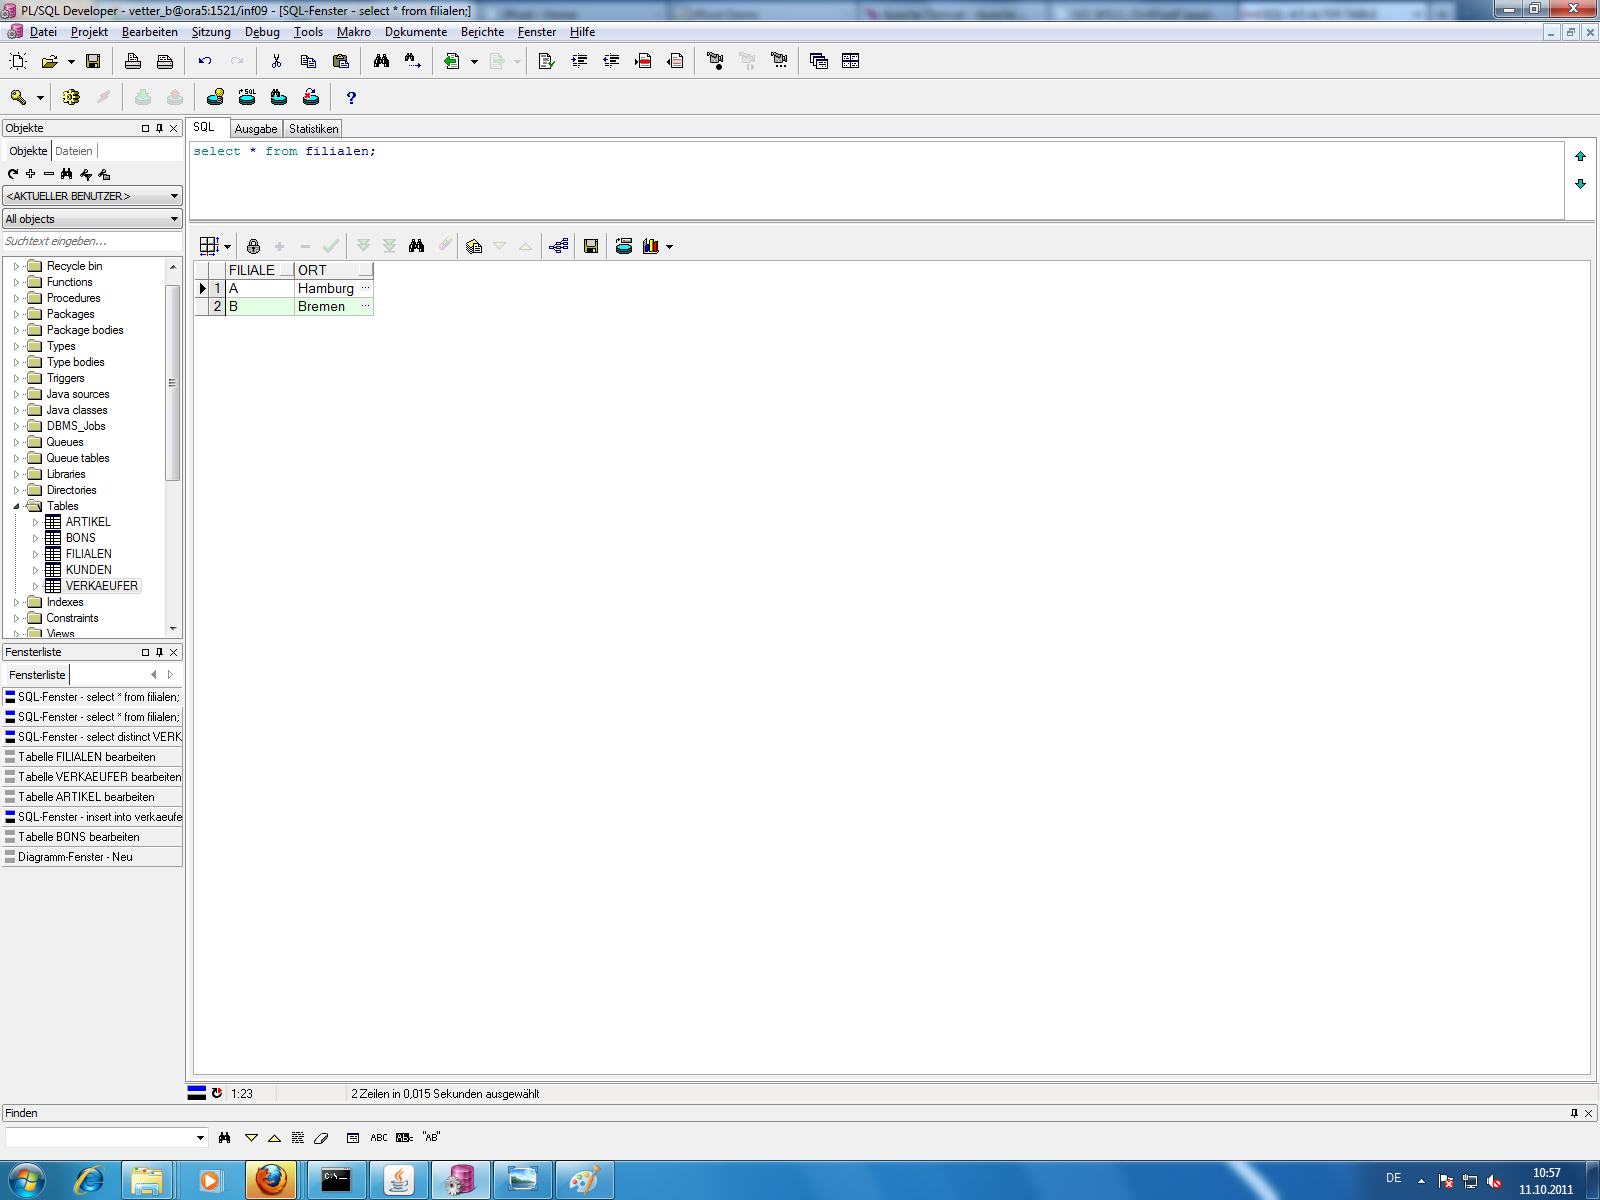
\includegraphics{screenshots/filialen.png}
  \caption{Tabelle Filialen}
\end{figure}

\begin{figure}
  \centering
  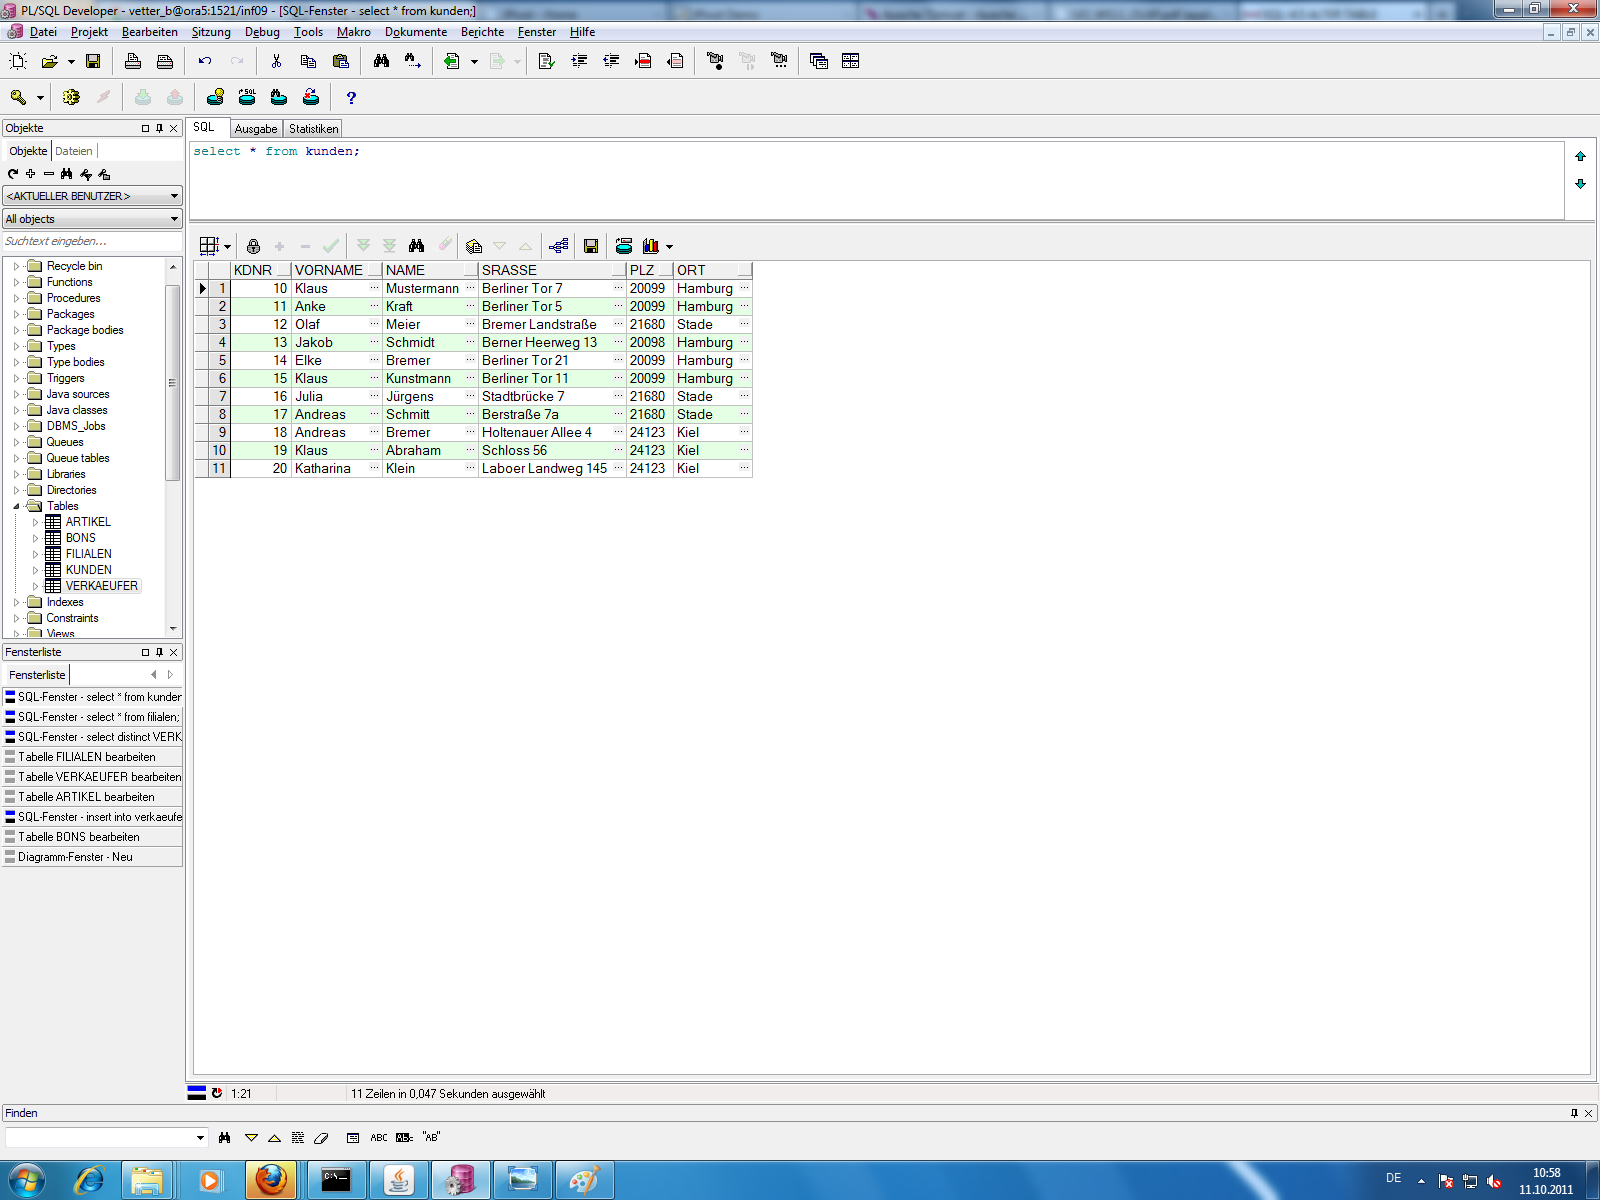
\includegraphics{screenshots/kunden.png}
  \caption{Tabelle Kunden}
\end{figure}

\begin{figure}
  \centering
  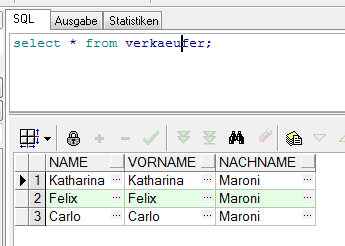
\includegraphics{screenshots/verkaeufer.png}
  \caption{Tabelle Verkaeufer}
\end{figure}

\chapter{Teil C}

\begin{lstlisting}[caption={XML-Schema}]
<?xml version="1.0"?>
<Schema name="BonDaten">
  <Cube name="BonDaten">
    <Table name="BONS"/>
    
    <Dimension name="ARTIKEL" foreignKey="ARTIKEL">
      <Hierarchy hasAll="true" allMemberName="Alle Artikel" primaryKey="ARTNR">
        <Table name="ARTIKEL"/>
        <Level name="ARTIKELNAME" column="ARTNAME" uniqueMembers="true"/>
      </Hierarchy>
    </Dimension>
    
    <Dimension name="FILIALEN" foreignKey="FILIALE">
      <Hierarchy hasAll="true" allMemberName="Alle Filialen" primaryKey="FILIALE">
        <Table name="FILIALEN"/>
        <Level name="FILALE" column="FILIALE" uniqueMembers="true"/>
      </Hierarchy>
    </Dimension>
    
    <Dimension name="KUNDEN" foreignKey="KUNDE">
      <Hierarchy hasAll="true" allMemberName="Alle Kunden" primaryKey="KDNR">
        <Table name="KUNDEN"/>
        <Level name="NAME" column="NAME" uniqueMembers="true">
          <Property name="Vorname" column="VORNAME"/>
          <Property name="Strasse" column="SRASSE"/>
          <Property name="PLZ" column="PLZ"/>
          <Property name="Ort" column="ORT"/>
        </Level>
      </Hierarchy>
    </Dimension>
    
    <Dimension name="VERKAEUFER" foreignKey="VERKAEUFER">
      <Hierarchy hasAll="true" allMemberName="Alle Verkaeufer" primaryKey="NAME">
        <Table name="VERKAEUFER"/>
        <Level name="NAME" column="NAME" uniqueMembers="true"/>
      </Hierarchy>
    </Dimension>

    <Measure name="Preis Total" column="PREIS" aggregator="sum" formatString="#.###"/>
    <Measure name="Count Total" column="PREIS" aggregator="count" formatString="####"/>
    <Measure name="AVG Total" column="PREIS" aggregator="avg" formatString="#.###"/>
  </Cube>
</Schema>
\end{lstlisting}

Die Dimensionen sind entsprechend den SQL-Tabellen benannt.
Daher ist die Abbildung des XML-Schemas auf die Tabellen trivial.

\begin{lstlisting}[caption={Query 1}]
  select {
    [Measures].[Preis Total],
    [Measures].[Count Total],
    [Measures].[AVG Total]
  } on columns, {(
    [FILIALEN].[Alle Filialen],
    [VERKAEUFER].[Alle Verkaeufer],
    [ARTIKEL].[Alle Artikel],
    [KUNDEN].[Alle Kunden]
  )}
  on rows from [BonDaten]
\end{lstlisting}

Diese Query gibt alle im XML-Schema definierten Dimensionen und Attribute wieder.

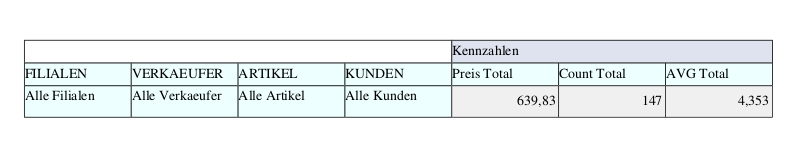
\includegraphics[width=\textwidth]{queries/query1.png}

\begin{lstlisting}[caption={Query 2}]
  select Hierarchize(Union({
    [FILIALEN].[Alle Filialen]
  }, [FILIALEN].[Alle Filialen].Children)) ON COLUMNS, {
    [Measures].[Preis Total],
    [Measures].[Count Total],
    [Measures].[AVG Total]
  } ON ROWS from [BonDaten]
\end{lstlisting}

Diese Query fragt den Umsatz, die Anzahl der verkauften Einheiten und den durchschnittlichen Verkaufspreis pro Filiale ab.

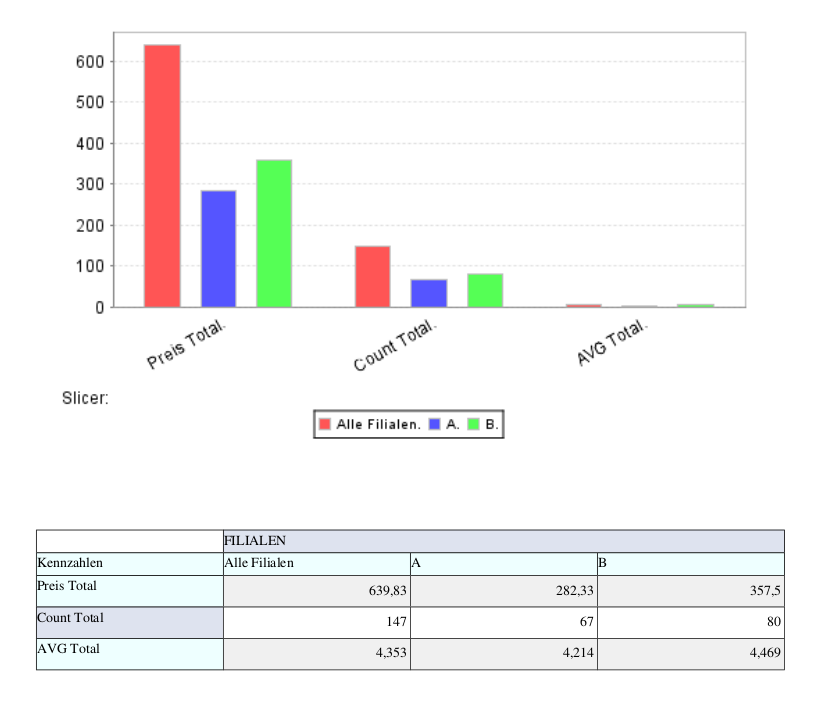
\includegraphics[width=\textwidth]{queries/query2.png}

\end{document}

